\documentclass{article}
\usepackage{graphicx} % Required for inserting images
\usepackage{geometry}
\usepackage{circuitikz}
\usepackage{siunitx}
\usepackage{CJKutf8}
\usepackage{amsmath}
\usepackage{amssymb}
\usepackage{caption}
\usepackage{float}
\usepackage{subcaption}
\geometry{top=5mm, left=30mm, a4paper}

\title{Common-Source Amplifier Analysis Prelab}
\author{梁程捷 (B11901136), 吳奕娃 (B11901080)}
\date{}


\begin{document}
\begin{CJK*}{UTF8}{bkai}

\maketitle


\begin{figure}[h]
    \begin{center}
    
        \begin{subfigure}[b]{0.25\textwidth}
            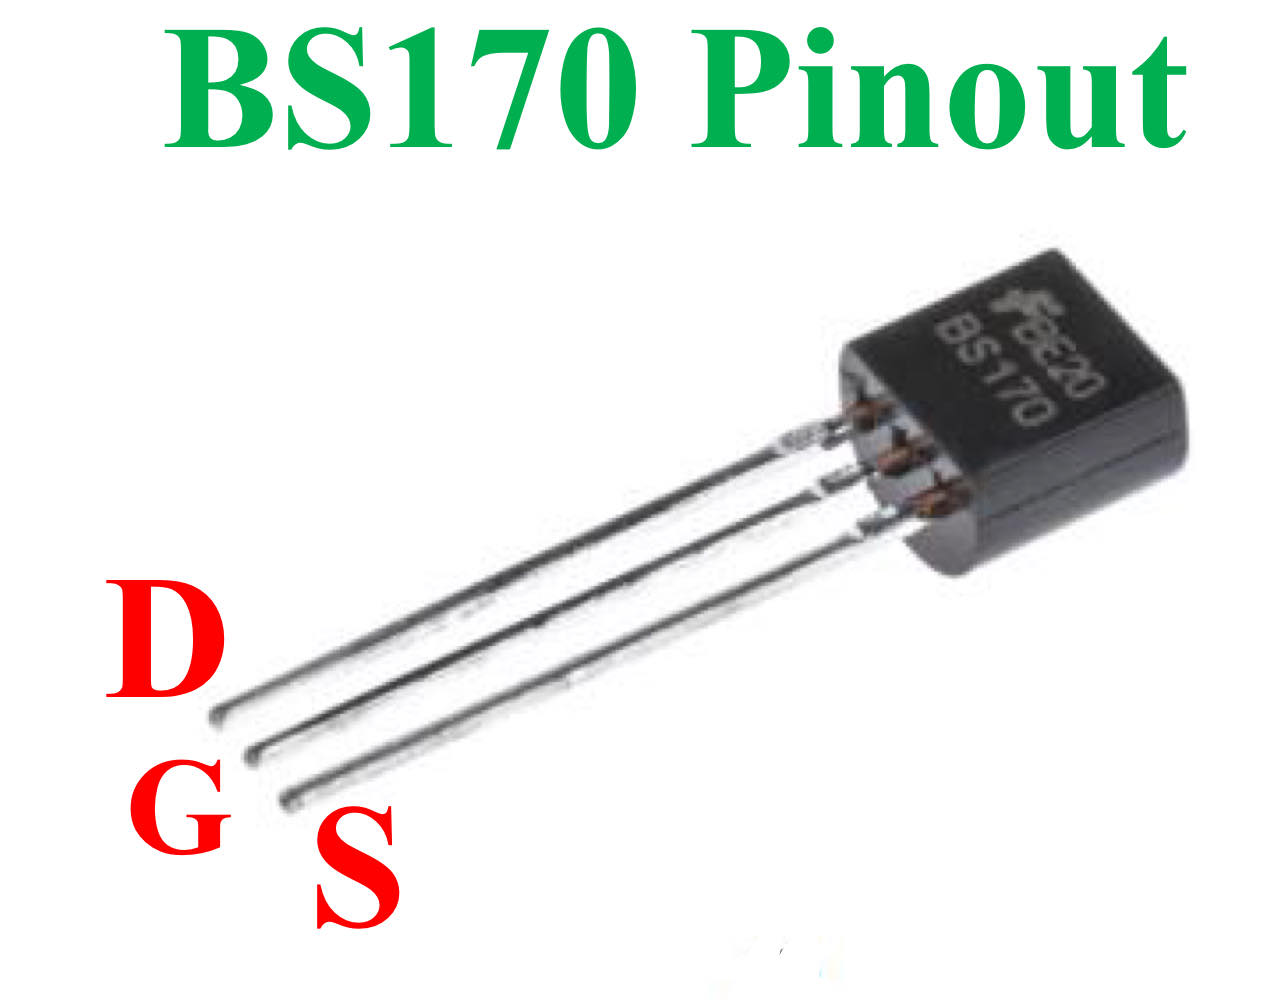
\includegraphics[width=\textwidth]{BS170_pinout.jpg}
            \caption{BS170 pinout}
        \end{subfigure}
        ~
        \begin{subfigure}[b]{0.7\textwidth}
            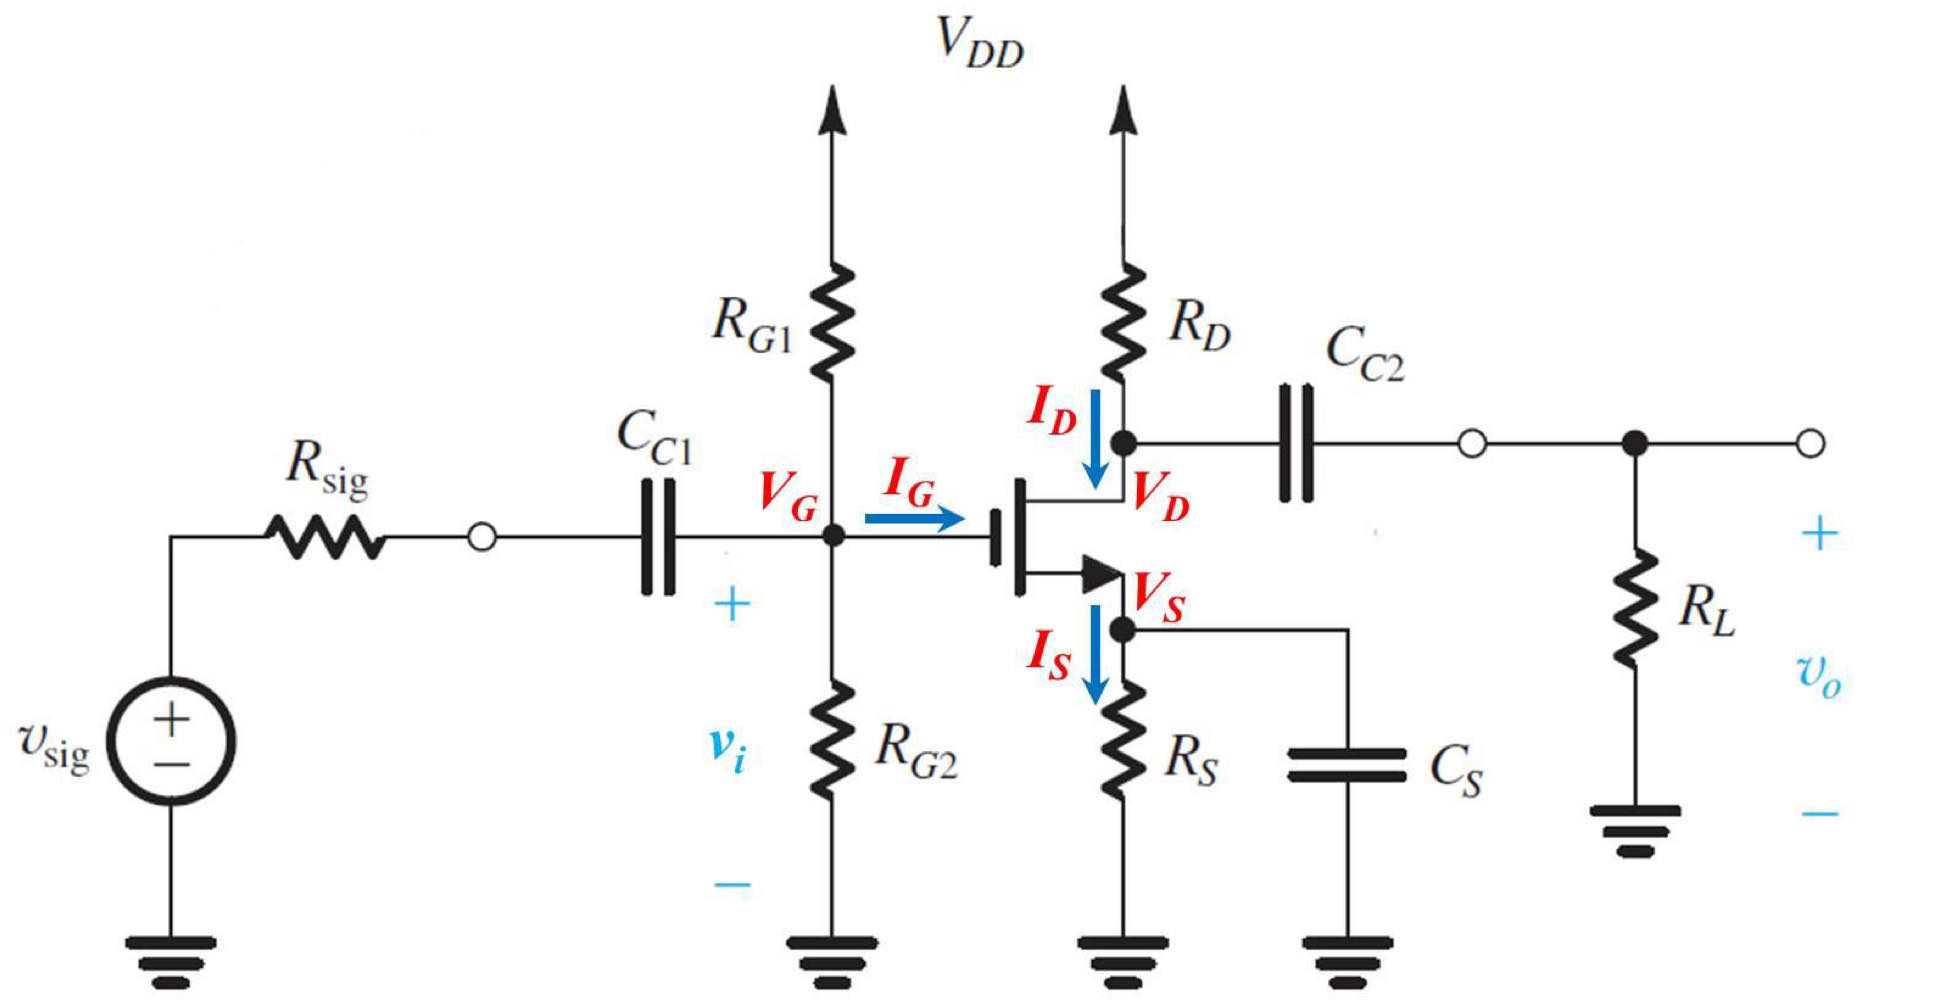
\includegraphics[width=\textwidth]{cs_amp_circuit.jpg}
            \caption{CS-Amplifier circuit}
        \end{subfigure}
    \end{center}
\end{figure}

\textbf{FET model: BS170}\\
\textbf{Voltage source:} $V_{DD} = +15$ \unit{\volt}; $v_{sig} = 0.2 \sin(2 \pi f t)$, $f = 200$ \unit{\hertz} $\sim$ 500 \unit{\kilo\hertz}\\
\textbf{Resistors: }$R_{G1} = R_{G2} = 1$ \unit{\mega\ohm}; $R_D = R_S = R_L = 10$ \unit{\kilo\ohm}; $R_{sig} = 100$ \unit{\kilo\ohm}\\
\textbf{Capacitors: }$C_{C2} = C_S = 0.1$ \unit{\micro\farad} (104); $C_{C1} = 0.01$ \unit{\micro\farad} (103)\\

\section*{DC analysis}
Measure $V_G$, $V_D$, $V_S$, $I_G$, $I_D$ and $I_S$

\section*{Small-signal analysis}
At a specific frequency ($f = 1$ \unit{\kilo\hertz} $\sim$ 20 \unit{\kilo\hertz}),\\
\textbf{measure} $\displaystyle{\left\lvert \frac{v_o}{v_{sig}}\right\rvert}$, $\displaystyle{\left\lvert \frac{v_o}{v_i}\right\rvert}$ \textbf{\underline{WITH}} and \textbf{\underline{WITHOUT}} $C_S$ respectively.\\
Record the input and output waveforms in \textbf{Y-t mode}.\vspace{2mm}\\
Make a conclusion according to the experimental result.


\end{CJK*}
\end{document}